%\section{Potential scenarios where our method can be useful}

%\textbf{N-body Simulations:} This experiment is introduced in \cite{kipf2018neural} and adapted in \cite{fuchs2020se}. N-particles embedded in a 3-dimensional with either negative or positive charge exert repulsive or attractive forces on each other. The algorithm has to predict the relative position of these particles after a given number of time steps. Since the relative positions are invariant to rotations and translations on set of particles our algorithm can benefit from it. The relative position of the particles would be the $X$ coordinates in our algorithm. For more information about the dataset refer to Experiment 4.1 in \cite{fuchs2020se}. 

%\textbf{QM9:} QM9 is a \cite{ramakrishnan2014quantum} publicly available chemical property prediction dataset for molecules with up to 29 atoms per molecule. The position of each atom is provided in the dataset. The atom positions would be the coordinates $X$ in our algorithm. Other molecule datasets where our algorithm could be used are MD17 \cite{chmiela2017machine} and ISO17 \url{http://www.quantum-machine.org/}.


%\textbf{Graph Autoencoder:} In the next section we show how our algorithm can also be used for graph autoencoding. We can randomly assign a n-dimensional particle to each node of the graph and then express the edges of our graph as a similarity measure on pairs of particles. Following this approach we show how our a graph autoencoder built from our equivariant equations overcomes other algorithms when embedding and reconstructing a graph into a low dimensional space. 




%\textbf{Graph Visualization:} Comparison to T-SNE.

%\textbf{Protein folding:} Generating 3D shape proteins from its sequence \cite{eismann2020protein}. As done in Alpha Fold or this workshop paper from NeurIPS \cite{eismann2020protein} uses Tensor Field Networks to generate the 3D shape of a protein beucase they are translation and rotation equivariant.



%\textbf{Limitations:} Experiment 5.1 from Tensor Field Networks \cite{thomas2018tensor} would be the only limitation.  (Pending to explain why).


\section{Experiments}

\subsection{Modelling a dynamical system | N-body system } \label{sec:experiment_n_body}

In a dynamical system a function defines the time dependence of a point or set of points in a geometrical space. Modelling these complex dynamics is crucial in a variety of applications such as control systems \cite{chua2018deep}, model based dynamics in reinforcement learning \cite{nagabandi2018neural}, and physical systems simulations \cite{grzeszczuk1998neuroanimator, watters2017visual}. In this experiment we forecast the positions for a set of particles which are modelled by simple interaction rules, yet can exhibit complex dynamics.

Similarly to \cite{fuchs2020se}, we extended the Charged Particles N-body experiment from \cite{kipf2018neural} to a 3 dimensional space. The system consists of 5 particles that carry a positive or negative charge and have a position and a velocity associated in 3-dimensional space. The system is controlled by physic rules: particles are attracted or repelled depending on their charges. This is an equivariant task since rotations and translations on the input set of particles result in the same transformations throughout the entire trajectory. 


\textbf{Dataset}: We sampled 3.000 trajectories for training, 2.000 for validation and 2.000 for testing. Each trajectory has a duration of 1.000 timesteps. For each trajectory we are provided with the initial particle positions $\rmp^{(0)}=\{ \rmp^{(0)}_1, \dots \rmp^{(0)}_5 \} \in \mathbb{R}^{5 \times 3}$, their initial velocities $\rmv^{(0)}=\{ \rmv^{(0)}_1, \dots \rmv^{(0)}_5 \} \in \mathbb{R}^{5 \times 3}$ and their respective charges $\mathbf{c} = \{c_1, \dots c_5\} \in \{-1, 1\}^5$. The task is to estimate the positions of the five particles after 1.000 timesteps. We optimize the averaged Mean Squared Error of the estimated position with the ground truth one.


\textbf{Implementation details:} In this experiment we used the extension of our model that includes velocity from section \ref{sec:method_velocity}. We input the position $\rmp^{(0)}$ as the first layer coordinates $\rmx^0$ of our model and the velocity $\rmv^{(0)}$ as the initial velocity in Equation \ref{eq:egnn_velocity}, the norms $\|\rmv_i^{(0)} \|$ are also provided as features to $\rmh_i^0$ through a linear mapping. The charges are input as edge attributes $a_{ij} = c_i c_j$. The model outputs the last layer coordinates $\rmx^L$ as the estimated positions.
%We used 4 layers in our EGNN and 64 features for the hidden layers. As non-linearity we used the Swish activation function \cite{ramachandran2017searching}. 
We compare our method to its non equivariant Graph Neural Network (GNN) cousin, and the equivariant methods: Radial Field \cite{kohler2019equivariant_workshop}, Tensor Field Networks and the SE(3) Transformer. All algorithms are composed of 4 layers and have been trained under the same conditions, batch size 100, 10.000 epochs, Adam optimizer, the learning rate was tuned independently for each model. We used 64 features for the hidden layers in the Radial Field, the GNN and our EGNN. As non-linearity we used the Swish activation function \cite{ramachandran2017searching}. For TFN and the SE(3) Transformer we swept over different number of vector types and features and chose those that provided the best performance. Further implementation details are provided in Appendix \ref{sec:appendix_implementation_dynamical}. A Linear model that simply considers the motion equation $\rmp^{(t)} = \rmp^{(0)} + \rmv^{(0)}t$ is also included as a baseline. We also provide the average forward pass time in seconds for each of the models for a batch of 100 samples in a GTX 1080 Ti GPU.
%\textbf{Preserving equivariance to $\rmv_i$}: In this experiment we want to input some initial conditions $\rmp_i$ and $\rmv_i$. Inputting $\rmp_i$ is straightforward, it can be directly inputted to the first line of equation \ref{eq:proposed_model} as the equivariant coordinates $\rmx_i^{(0)}$. Regarding the initial conditions $\rmv_i$, it would also be benefitial to also preserve equivariance to rotations ans translations on them. To achieve this we preserve a change of basis that keeps the coordinates $\mathbf{v}_i$ equivariant to rotations and translation. This change of basis can be applicable to any other vector whose equivariance we want to preserve and it is not restricted to only velocity.

%The procedure is very simple. We just project each particle's velocity $\rmv_i$ from each node $i$, into the normalized vectors $(x_j - x_i)$ associated to each of its neighbors $j \in \mathcal{N}(i)$. The operation will be as follows:
%\begin{equation}
%    v_{ij} = \rmv_i \cdot \frac{\x_j - %\x_i}{\lVert \x_j - \x_i\rVert}
%\end{equation}
%The scalar value $v_{ij}$ is the projection of the vector $\rmv_i$ on the base $\frac{\x_j - \x_i}{\lVert \x_j - \x_i\rVert}$. We input these scalar values as an attribute $e_{ij}$ in equation \ref{eq:proposed_model} for each edge. The value of these scalar will be invariant to rotations and translations on the set of particles (prove it in the appendix).


\begin{table}[h] 
  \centering
  \begin{tabular}{lcc}
  \toprule
    Method & MSE & Forward time (s)  \\
    \midrule
    Linear & 0.0819 & .0001  \\
       SE(3) Transformer & 0.0244 & .1346  \\ 
       Tensor Field Network & 0.0155 & .0343  \\ 
        Graph Neural Network &  0.0107 & .0032  \\ 
       Radial Field & 0.0104 & .0039  \\
    \textbf{EGNN} & \textbf{0.0071}  & .0062\\ 
    \bottomrule
  \end{tabular}
  \caption{Mean Squared Error for the future position estimation in the N-body system experiment, and forward time in seconds for a batch size of 100 samples running in a GTX 1080Ti GPU.}
  \label{table:n_body}
\end{table}
\vspace{-5pt}

\textbf{Results}
As shown in Table \ref{table:n_body} our model significantly outperforms the other equivariant and non-equivariant alternatives while still being efficient in terms of running time. It reduces the error with respect to the second best performing method by a $32\%$. In addition it doesn't require the computation of spherical harmonics which makes it more time efficient than Tensor Field Networks and the SE(3) Transformer.



\begin{figure}[h!]
\begin{center}
\centerline{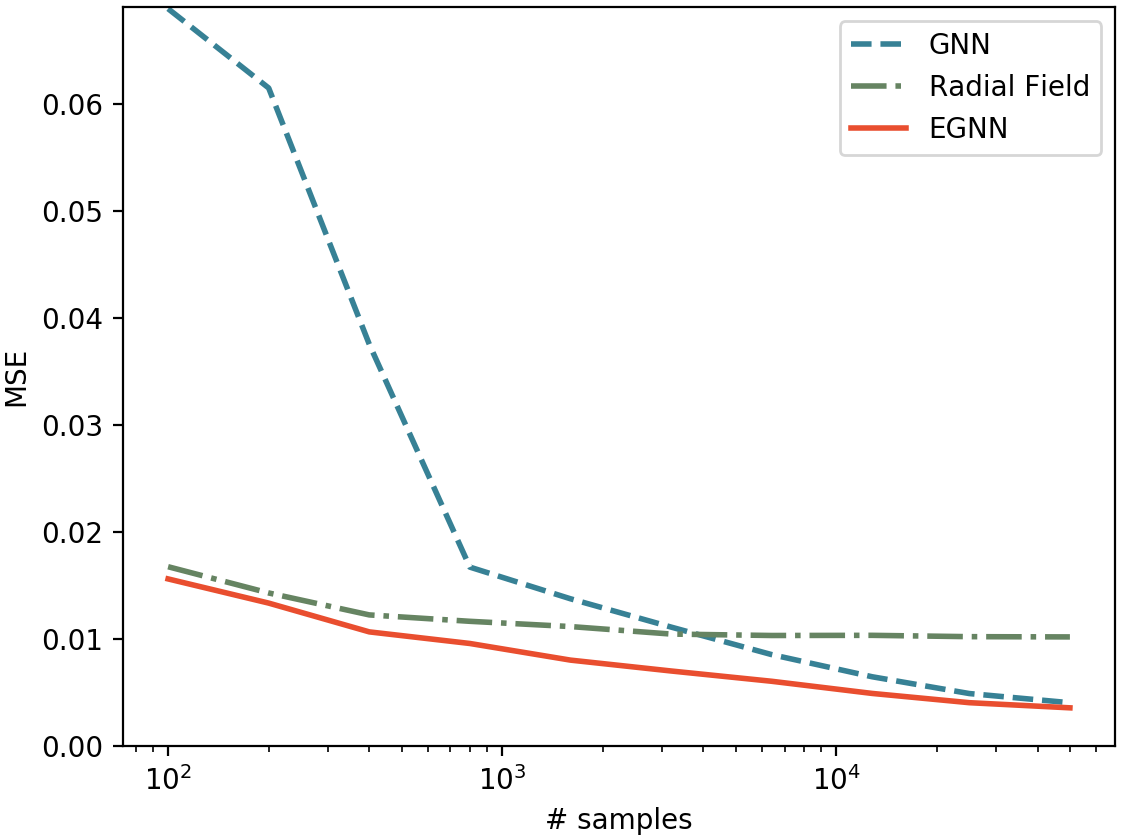
\includegraphics[width=0.8\columnwidth]{Figures/n_body.png}}
%\vspace{-5pt}
\caption{Mean Squared Error in the N-body experiment for the Radial Field, GNN and EGNN methods when sweeping over different amounts of training data.}
\label{fig:n_body_figure}
\end{center}
\vskip -0.25in
\end{figure}


\textbf{Analysis for different number of training samples:} We want to analyze the performance of our EGNN in the small and large data regime. In the following, we report on a similar experiment as above, but instead of using 3.000 training samples we generated a new training partition of 50.000 samples and we sweep over different amounts of data from 100 to 50.000 samples. We compare the performances of our EGNN vs its non-equivariant GNN counterpart and the Radial Field algorithm. Results are presented in Figure \ref{fig:n_body_figure}. Our method outperforms both Radial Field and GNNs in the small and large data regimes. This shows the EGNN is more data efficient than GNNs since it doesn't require to generalize over rotations and translations of the data while it ensembles the flexibility of GNNs in the larger data regime. Due to its high model bias, the Radial Field algorithm performs well when data is scarce but it is unable to learn the subtleties of the dataset as we increase the training size. In summary, our EGNN benefits from both the high bias of $\En$ methods and the flexibility of GNNs.


\subsection{Graph Autoencoder} \label{sec:expriment_autoencoder}



A Graph Autoencoder can learn unsupervised representations of graphs in a continuous latent space \cite{kipf2016variational, simonovsky2018graphvae}. In this experiment section we use our EGNN to build an Equivariant Graph Autoencoder. We will explain how Graph Autoencoders can benefit from equivariance and we will show how our method outperforms standard GNN autoencoders in the provided datasets. This problem is particularly interesting since the embedding space can be scaled to larger dimensions and is not limited to a 3 dimensional Euclidean space.

Similarly to the work of \cite{kipf2016variational} further extended by section 3.3 in \cite{liu2019graph}, our graph auto-encoder $\rmz = q(\mathcal{G})$ embeds a graph $\mathcal{G}$ into a set of latent nodes $\rmz = \{\rmz_1, \dots \rmz_M \} \in \mathbb{R}^{M \times n}$, where $M$ is the number of nodes and $n$ the embedding size per node. Notice this may reduce the memory complexity to store the graphs from $O(M^2)$ to $O(Mn)$ where $n$ may depend on $M$ for a certain approximation error tolerance. This differs from the variational autoencoder proposed in \cite{simonovsky2018graphvae} which embeds the graph in a single vector $\rmz \in \mathbb{R}^K$, which causes the reconstruction to be computationally very expensive since the nodes of the decoded graph have to be matched again to the ground truth. In addition to the introduced graph generation and representation learning methods, it is worth it mentioning that in the context of graph compression other methods \cite{candes2009exact} can be used.

More specifically, we will compare our Equivariant Graph Auto-Encoder in the task presented in \cite{liu2019graph} where a graph $\mathcal{G} = (\mathcal{V}, \mathcal{E})$ with node features $H \in \mathbb{R}^{M \times \text{nf}}$ and adjacency matrix $A \in \{0, 1\}^{M \times M}$ is embedded into a latent space $\rmz = q(H, A) \in \mathbb{R}^{M \times n}$. Following \cite{kipf2016variational, liu2019graph}, we are only interested in reconstructing the adjacency matrix $A$ since the datasets we will work with do not contain node features. The decoder $g(\cdot)$ proposed by \cite{liu2019graph} takes as input the embedding space $\rmz$ and outputs the reconstructed adjacency matrix $\hat{A} = g(\rmz)$, this decoder function is defined as follows:
\begin{equation} \label{eq:graph_decoder}
    \hat{A}_{ij} = g_e(\rmz_i, \rmz_j)=\frac{1}{1 + \mathrm{exp}(
w\left\|\rmz_{i}- \rmz_{j}\right\|^{2} + b
)}
\end{equation}

Where $w$ and $b$ are its only learnable parameters and $g_e(\cdot)$ is the decoder edge function applied to every pair of node embeddings. It reflects that edge probabilities will depend on the relative distances among node embeddings. The training loss is defined as the binary cross entropy between the estimated and the ground truth edges $\mathcal{L} = \sum_{ij}\mathrm{BCE}(\hat{A}_{ij}, A_{ij})$.


\textbf{The symmetry problem:} The above stated autoencoder may seem straightforward to implement at first sight but in some cases there is a strong limitation regarding the symmetry of the graph. Graph Neural Networks are convolutions on the edges and nodes of a graph, i.e. the same function is applied to all edges and to all nodes. In some graphs (e.g. those defined only by its adjacency matrix) we may not have input features in the nodes, and for that reason the difference among nodes relies only on their edges or neighborhood topology. Therefore, if the neighborhood of two nodes is exactly the same, their encoded embeddings will be the same too. A clear example of this is a cycle graph (an example of a 4 nodes cycle graph is provided in Figure \ref{fig:symmetric_cycle_graph}). When running a Graph Neural Network encoder on a node featureless cycle graph, we will obtain the exact same embedding for each of the nodes, which makes it impossible to reconstruct the edges of the original graph from the node embeddings. The cycle graph is a severe example where all nodes have the exact same neighborhood topology but these symmetries can be present in different ways for other graphs with different edge distributions or even when including node features if these are not unique.

\begin{figure}[h]
\begin{center}
\centerline{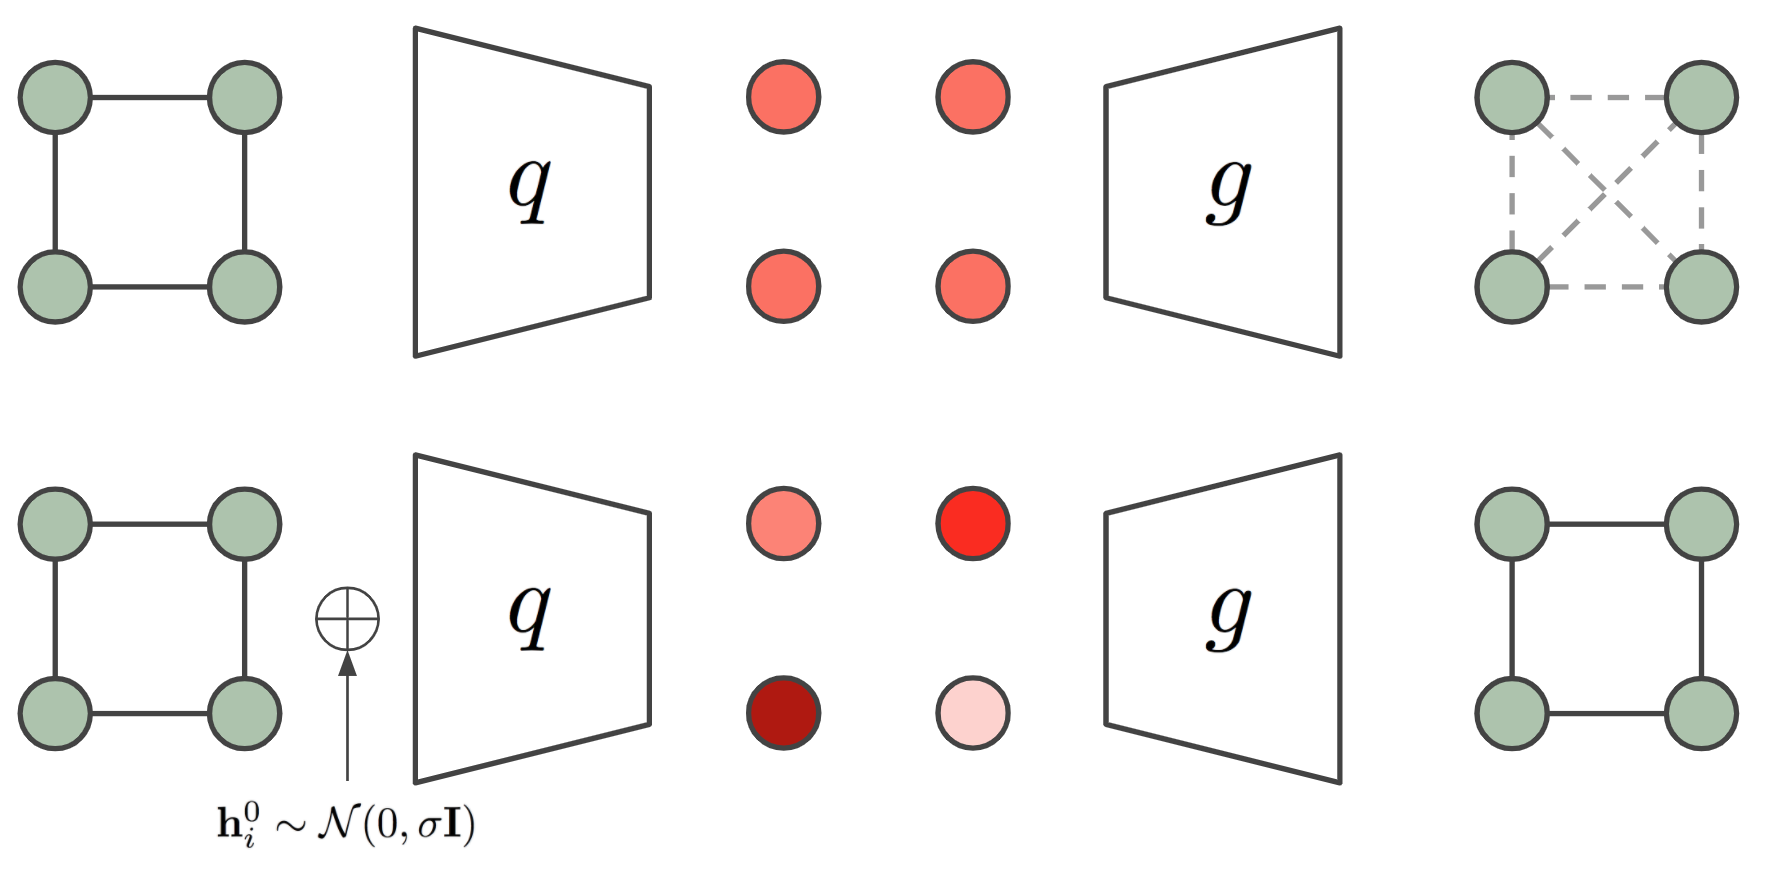
\includegraphics[width=0.7\columnwidth]{Figures/on_breakin_symmetry.png}}
\caption{Visual representation of a Graph Autoencoder for a 4 nodes cycle graph. The bottom row illustrates that adding noise at the input graph breaks the symmetry of the embedding allowing the reconstruction of the adjacency matrix.}
\label{fig:symmetric_cycle_graph}
\end{center}
\vskip -0.2in
\end{figure}




  \begin{figure*}[t]
    \centering
    \vspace{-.3cm}
    \begin{minipage}[c]{.59\textwidth}
    \begin{tabular}{lcccccc}
    \toprule
     & \multicolumn{3}{c}{Community Small} &   \multicolumn{3}{c}{Erdos\&Renyi}\\
    Encoder & BCE & \% Error & F1 & BCE & \% Error & F1 \\
    \midrule
    Baseline & - & 31.79 & .0000 & - & 25.13 & 0.000    \\
    GNN & 6.75 & 1.29 & 0.980 & 14.15 & 4.62 & 0.907  \\
    Noise-GNN & 3.32 & 0.44 & 0.993 & 4.56 & 1.25 & 0.975  \\
    %Noise-GNN*  & - & 0.57  & - & 3.25\\
    Radial Field & 9.22 & 1.19 & 0.981 & 6.78 & 1.63 & 0.968 \\
    EGNN & \textbf{2.14} & \textbf{0.06} & \textbf{0.999} & \textbf{1.65} & \textbf{0.11} & \textbf{0.998}  \\
    \bottomrule
    \end{tabular}
    \end{minipage}\begin{minipage}[c]{.4\textwidth}\vspace{.3cm}
    \centering
    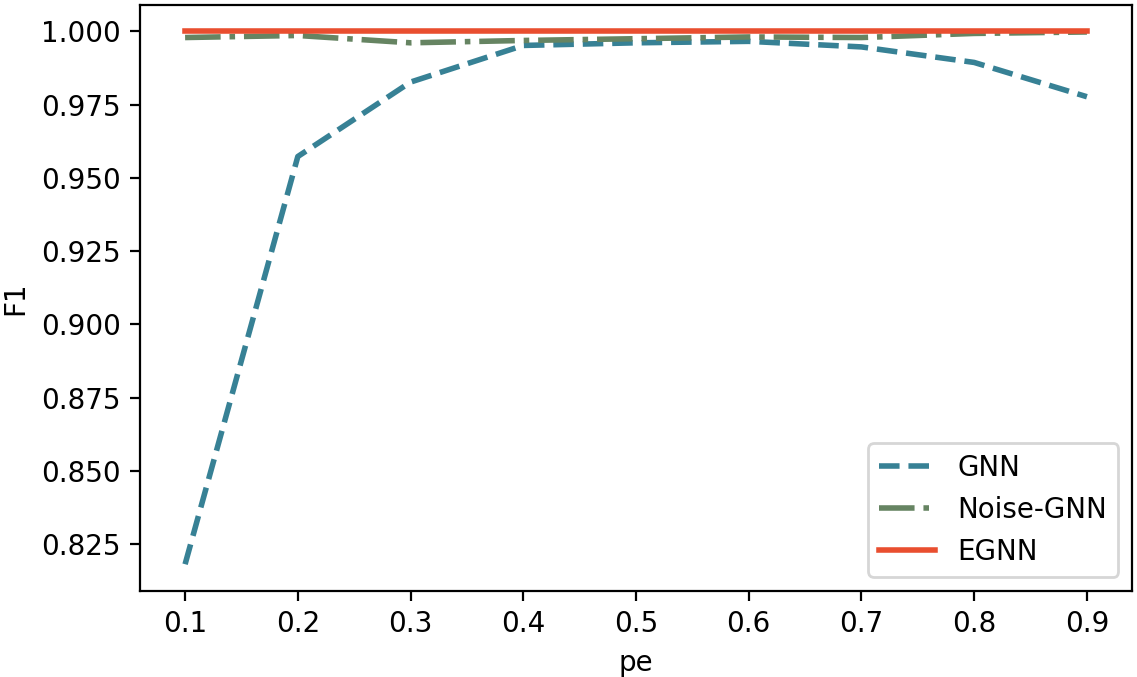
\includegraphics[width=0.99\textwidth]{Figures/sweep_pe.png}
    \end{minipage}
    \captionlistentry[figure]{}
    %\captionsetup{labelformat=andtable}
    \vspace{-.2cm}
    \caption{In the Table at the left we report the Binary Cross Entropy, \% Error and F1 scores for the test partition on the Graph Autoencoding experiment in the Community Small and Erdos\&Renyi datasets. In the Figure at the right, we report the F1 score when overfitting a training partition of 100 samples in the Erdos\&Renyi dataset for different values of sparsity $p_e$. The GNN is not able to successfully auto-encode sparse graphs (small $p_e$ values) for the Erdos\&Renyi dataset even when training and testing on the same small subset.}
    \vspace{-.2cm}
    \label{table:autoencoder_results}
  \end{figure*}


An ad-hoc method to break the symmetry of the graph is introduced by \cite{liu2019graph}. This method introduces noise sampled from a Gaussian distribution into the input node features of the graph $\rmh_i^{0} \sim \mathcal{N}(\mathbf{0}, \sigma\mathbf{I})$. This noise allows different representations for all node embeddings and as a result the graph can be decoded again, but it comes with a drawback, the network has to generalize over the new introduced noise distribution. Our Equivariant Graph Autoencoder will remain translation and rotation equivariant to this sampled noise which we find makes the generalization much easier. Another way of looking at this is considering the sampled noise makes the node representations go from structural to positional  \cite{srinivasan2019equivalence} where $\En$ equivariance may be beneficial. In our case we will simply input this noise as the input coordinates $\rmx^{0} \sim \mathcal{N}(\mathbf{0}, \sigma\mathbf{I}) \in \mathbb{R}^{M \times n}$ of our EGNN which will output an equivariant transformation of them $\rmx^L$, this output will be used as the embedding of the graph (i.e. $\rmz = \rmx^L$) which is the input to the decoder from Equation \ref{eq:graph_decoder}.




\textbf{Dataset:} We generated community-small graphs \cite{you2018graphrnn, liu2019graph} by running the original code from \cite{you2018graphrnn}. These graphs contain $12\leq M \leq20$ nodes. We also generated a second dataset using the Erdos\&Renyi generative model \cite{bollobas2001random} sampling random graphs with an initial number of $7\leq M \leq16$ nodes and edge probability $p_e=0.25$. We sampled $5.000$ graphs for training, $500$ for validation and $500$ for test for both datasets. Each graph is defined as and adjacency matrix $A \in \{0, 1\}^{M \times M}$.

\textbf{Implementation details:} Our Equivariant Graph Auto-Encoder is composed of an EGNN encoder followed by the decoder from Equation \ref{eq:graph_decoder}. The graph edges $A_{ij}$ are input as edge attributes $a_{ij}$ in Equation \ref{eq:method_edge}. The noise used to break the symmetry is input as the coordinates $\rmx^0 \sim \mathcal{N(\mathbf{0}, \sigma\mathbf{I})} \in \mathbb{R}^{M \times n}$ in the first layer and $\rmh^0$ is initialized as ones since we are working with featureless graphs. As mentioned before, the encoder outputs an equivariant transformation on the coordinates which is the graph embedding and input to the decoder $\rmz = \rmx^L \in \mathbb{R}^{M\times n}$. We use $n=8$ dimensions for the embedding space. We compare the EGNN to its GNN cousin, we also compare to Noise-GNN which is an adaptation of our GNN to match the setting from \cite{liu2019graph}, and we also include the Radial Field algorithm as an additional baseline. All four models have 4 layers, 64 features for the hidden layers, the Swish activation function as a non-linearity and they were all trained for 100 epochs using the Adam optimizer and learning rate $10^{-4}$. More details are provided in Appendix \ref{sec:appendix_implementation_graph_autoencoders}. Since the number of nodes is larger than the number of layers, the receptive field of a GNN may not comprise the whole graph which can make the comparison unfair with our EGNN. To avoid this limitation, all models exchange messages among all nodes and the edge information is provided as edge attributes $a_{ij} = A_{ij}$ in all of them.


\textbf{Results:} In the table from Figure \ref{table:autoencoder_results} we report the Binary Cross Entropy loss between the estimated and ground truth edges, the \% Error which is defined as the percentage of wrong predicted edges with respect to the total amount of potential edges, and the F1 score of the edge classification, all numbers refer to the test partition. We also include a "Baseline" that predicts all edges as missing $\hat{A}_{ij}=0$. The standard GNN seems to suffer from the symmetry problem and provides the worst performance. When introducing noise (Noise-GNN), both the loss and the error decrease showing that it is actually useful to add noise to the input nodes. Finally, our EGNN remains $\En$ equivariant to this noise distribution and provides the best reconstruction with a $0.11\%$ error in the Erdos\&Renyi dataset and close to optimal $0.06\%$ in the Community Small dataset. A further analysis of the reconstruction error for different $n$ embedding sizes is reported in Appendix \ref{sec:appendix_graph_autoencoder}. 


\begin{table*}[th]
  \centering
  \begin{tabular}{l c c c c c c c c c c c c}
  \toprule
    Task & $\alpha$ & $\Delta \varepsilon$ & $\varepsilon_{\mathrm{HOMO}}$ & $\varepsilon_{\mathrm{LUMO}}$ & $\mu$ & $C_{\nu}$ & $G$ & $H$ & $R^2$ & $U$ & $U_0$ & ZPVE \\
    Units & bohr$^3$ & meV & meV & meV & D & cal/mol K & meV & meV & bohr$^3$ & meV & meV & meV \\
    \midrule
    %WaveScatt & .160 & 3 & 4 & 5 & 6 & 7 & 8 & 9 & 10 & 11 & 12 & 13 \\
    NMP & .092 & 69 & 43 & 38 & .030 & .040 & 19 & 17 & .180 & 20 & 20 & 1.50 \\
    Schnet & .235 & 63 & 41 & 34 & .033 & .033 & 14 & 14 & .073 & 19 & 14 & 1.70 \\
    Cormorant & .085 & 61 & 34 & 38 & .038 & .026 & 20 & 21 & .961 & 21 & 22 & 2.03  \\
    L1Net & .088 & 68 & 46 & 35 & .043 & .031 & 14 & 14 & .354 & 14 & 13 &  1.56\\
    
    LieConv & .084 & 49 & 30 & 25 & .032 & .038 & 22 & 24 & .800 & 19 & 19 & 2.28 \\
    DimeNet++* & .044 & 33 & 25 & 20 & .030 & .023 & 8 & 7 & .331 & 6 & 6 & 1.21  \\
    TFN & .223 & 58 & 40 & 38 & .064 & .101 & - & - & - & - & - & - \\
    SE(3)-Tr. & .142 & 53 & 35 & 33 & .051 & .054 & - & - & - & - & - & -  \\
    \midrule
    EGNN & .071  & 48 & 29 & 25 & .029 & .031 & 12 & 12 & .106 & 12 & 11 & 1.55  \\
    \bottomrule
  \end{tabular}
  \caption{Mean Absolute Error for the molecular property prediction benchmark in QM9 dataset. *DimeNet++ uses slightly different train/val/test partitions than the other papers listed here.}
  \label{tab:qm9}
\end{table*}


\textbf{Overfitting the training set:} We explained the symmetry problem and we showed the EGNN outperforms other methods in the given datasets. Although we observed that adding noise to the GNN improves the results, it is difficult to exactly measure the impact of the symmetry limitation in these results independent from other factors such as generalization from the training to the test set. In this section we conduct an experiment where we train the different models in a subset of 100 Erdos\&Renyi graphs and embedding size $n=16$ with the aim to overfit the data. We evaluate the methods on the training data. In this experiment the GNN is unable to fit the training data properly while the EGNN can achieve perfect reconstruction and Noise-GNN close to perfect. We sweep over different $p_e$ sparsity values from $0.1$ to $0.9$ since the symmetry limitation is more present in very sparse or very dense graphs. We report the F1 scores of this experiment in the right plot of Figure \ref{table:autoencoder_results}.


In this experiment we showed that $\En$ equivariance improves performance when embedding graphs in a continuous space as a set of nodes in dimension $n$. Even though this is a simple reconstruction task, we think this can be a useful step towards generating graphs or molecules where often graphs (i.e. edges) are decoded as pairwise distances or similarities between nodes e.g. \cite{kipf2016variational, liu2019graph, grover2019graphite}, and these metrics (e.g. eq. \ref{eq:graph_decoder}) are $\En$ invariant. Additionally this experiment also showed that our method can successfully perform in a $\En$ equivariant task for higher dimensional spaces where $n>3$.




\subsection{Molecular data | QM9}
The QM9 dataset \cite{ramakrishnan2014quantum} has become a standard in machine learning as a chemical property prediction task. The QM9 dataset consists of small molecules represented as a set of atoms (up to 29 atoms per molecule), each atom having a 3D position associated and a five dimensional one-hot node embedding that describe the atom type (H, C, N, O, F). The dataset labels are a variety of chemical properties for each of the molecules which are estimated through regression. These properties are invariant to translations, rotations and reflections on the atom positions.
Therefore those models that are E(3) invariant are highly suitable for this task. 

We imported the dataset partitions from \cite{anderson2019cormorant}, 100K molecules for training, 18K for validation and 13K for testing. A variety of 12 chemical properties were estimated per molecule. We optimized and report the Mean Absolute Error between predictions and ground truth.

\textbf{Implementation details:} Our EGNN receives as input the 3D coordinate locations of each atom which are provided as $\rmx_i^0$ in Equation \ref{eq:method_edge} and an embedding of the atom properties which is provided as input node features $\rmh_i^0$.  Since this is an invariant task and also $\rmx^0$ positions are static, there is no need to update the particle's position $\rmx$ by running Equation \ref{eq:method_coords} as we did in previous experiments. Consequently, we tried both manners and we didn't notice any improvement by updating $\rmx$. When not updating the particle's position (i.e. skipping Equation \ref{eq:method_coords}), our model becomes $\mathrm{E}(n)$ invariant, which is analogous to a standard GNN where all relative squared norms between pairs of points $\| \rmx_i - \rmx_j \|^2$ are inputted to the edge operation (eq. \ref{eq:method_edge}). Additionally, since we are not provided with an adjacency matrix and molecules can scale up to 29 nodes, we use the extension of our model from Section \ref{sec:edges_inference} that infers a soft estimation of the edges. Our EGNN network consists of 7 layers, 128 features per hidden layer and the Swish activation function as a non-linearity. A sum-pooling operation preceded and followed by two layers MLPs maps all the node embeddings $\rmh^{L}$ from the output of the EGNN to the estimated property value. Further implementation details are reported in Appendix. \ref{sec:appendix_implementation}. We compare to NMP \cite{gilmer2017neural}, Schnet \cite{schutt2017schnet}, Cormorant \cite{anderson2019cormorant}, L1Net \cite{miller2020relevance}, LieConv \cite{finzi2020generalizing}, DimeNet++ \cite{klicpera2020fast}, TFN \cite{thomas2018tensor} and SE(3)-Tr. \cite{fuchs2020se}.

\textbf{Results} are presented in Table \ref{tab:qm9}. Our method reports very competitive results in all property prediction tasks while remaining relatively simple, i.e. not introducing higher order representations, angles or spherical harmonics. %state of the art in 9 out of 12 property predictions, and it is the second best performing method for the remaining 3 properties. 
Perhaps, surprisingly, we outperform other equivariant networks that consider higher order representations while in this task, we are only using type-0 representations (i.e. relative distances) to define the geometry of the molecules. In Appendix \ref{appendix:invariant_features} we prove that when only positional information is given (i.e. no velocity or higher order type features), then the geometry is completely defined by the norms in-between points up to $\En$-transformations, in other words, if two collections of points separated by $\En$ transformations are considered to be identical, then the relative norms between points is a unique identifier of the collection.
